
\documentclass[letterpaper, 10 pt, conference]{ieeeconf}  % Comment this line out if you need a4paper

%\documentclass[a4paper, 10pt, conference]{ieeeconf}      % Use this line for a4 paper

\IEEEoverridecommandlockouts

\overrideIEEEmargins                                      % Needed to meet printer requirements.

%In case you encounter the following error:
%Error 1010 The PDF file may be corrupt (unable to open PDF file) OR
%Error 1000 An error occurred while parsing a contents stream. Unable to analyze the PDF file.
%This is a known problem with pdfLaTeX conversion filter. The file cannot be opened with acrobat reader
%Please use one of the alternatives below to circumvent this error by uncommenting one or the other
%\pdfobjcompresslevel=0
%\pdfminorversion=4

% The following packages can be found on http:\\www.ctan.org
%\usepackage{natbib}
\usepackage{graphicx} % for pdf, bitmapped graphics files
\graphicspath{ {images/} }
%\usepackage{epsfig} % for postscript graphics files
\usepackage{mathptmx} % assumes new font selection scheme installed
\usepackage{times} % assumes new font selection scheme installed
\usepackage{amsmath} % assumes amsmath package installed
\usepackage{amssymb}  % assumes amsmath package installed
\usepackage[mathscr]{euscript}

\title{\LARGE \bf
Power Minimal Optimal Control for Quadrotor UAVs in Continuous Time
}


\author{Alexander B. Faustino and Timothy Bretl% <-this % stops a space
	\thanks{The authors are with the Department of Aerospace Engineering, Coordinated Science Laboratory, 
		University of Illinois at Urbana-Champaign, Champaign, IL 61801, USA
		\tt\small \{afausti2, tbretl\}@illinois.edu}%
}


\begin{document}

\maketitle
\thispagestyle{empty}
\pagestyle{empty}


%%%%%%%%%%%%%%%%%%%%%%%%%%%%%%%%%%%%%%%%%%%%%%%%%%%%%%%%%%%%%%%%%%%%%%%%%%%%%%%%

% !TeX root = ../main.tex

\begin{abstract}
	Determining an aircraft's velocity that maximizes its range or endurance is a long solved problem in aerodynamics and flight mechanics. However, due to the dynamic limitations of quadrotors a decade ago these solutions have been widely ignored in robotic applications. We present experimental validation that incorporating solutions derived from momentum analysis can increase a quadrotor's endurance by as much as 20\%. We focus on quadrotors with a camera payload and demonstrate the advantages of orbiting a point-of-interest rather than hovering above it.
\end{abstract}

\section{INTRODUCTION}
\label{intro}
% !TeX root = ../main.tex
 
The last decade has seen quadrotor helicopters explode in popularity. From an emerging unmanned aerial vehicle (UAV) concept to a prominent research and commercial platform \cite{kumar2012opportunities,hoffmann2007quadrotor} quadrotors have become the nearly ubiquitous aerial robot. Their relative low cost and the simplicity of their dynamics when near hover \cite{bouabdallah2004pid} has made them popular in numerous applications \cite{heng2015efficient,roberts2017submodular,frazzoli2002real}. 

No matter the application, if the quadrotor is autonomous, all its motion is occurring near hover. This condition introduces the quadrotor platform's greatest weakness, power efficiency. In \cite{kumar2012opportunities} Kumar et al. state that the power required for a quadrotor to maintain hover is approximately 200 W per kg. Additionally, due to current LiPo battery technology a quadrotor's battery can be 25-30\% of its total mass. These two purely harware constraints restrict the size of an area that can be explored, the number of images that can be captured by an onboard camera, the mass of potential payloads, etc.. The problem of quadrotor power efficiency therefore creates a practical limit on the platform's utility. 

Currently, most approaches to solving this problem can be classified in to three categories, listed in descending order of prevalence: 
\begin{enumerate}
	\item hardware focused optimization
	\item algorithm (software) focused optimization
	\item development of bio-inspired, hybrid systems
\end{enumerate}
Traditionally, the bulk of work done to increase quadrotor efficiency is in the first category. Efforts here consist mostly of reducing the weight of materials such as the airframe, sensors, and power electronics. The second category has grown in popularity in recent years due to the increased capabilities of onboard computers. The most common methods here involve incorporating vehicle power consumption in to cost functions of existing optimal planning and control algorithms. Finally, the third category often produces novel systems that increase efficiency by tranisitioning to another dynamic mode such as perching, walking, or rolling. In \cite{karydis2017energetics}, Karydis et al. provide a thorough review of some of the most promising work in all three categories. Category one and three are not addressed further in this paper as the scope falls entirely in category two.

In this paper we present a solution for finding quadrotor trajectories between two points in $\mathbb{R}^3$ that minimize the total amount of power required, $P_{tot}$, to complete. Our solution differs from current methods by being a continuous time solution and allowing for changes in altitude. The remainder of the paper is organized as follows: Section II broadly reviews similar approaches already in the literature; Section III describes the dynamic model of the quadrotor including power consumption; Section IV details the formulation of our optimal control problem; Section V presents the results from our experiments in simulation; and Section VI contains discussion of future work and conclusions from this work.

Determining an aerial vehicle's endurance is a common problem in flight mechanics. Solutions for fixed wing and rotor aircraft maximum endurance in steady, forward flight are well known and widely used \cite{anderson2005introduction,leishman2006principles}. Maximum endurance is achieved by traveling at the relative velocity, $V_\infty$, where the power required, $P_{req}$, to overcome the drag force, $D$, is at a minimum. We call this velocity $V_{me}$. 


\begin{figure}[ht]
    \label{QuadDiagram}
	\centering
	
\includegraphics[width=8cm]{placeholder-image.jpg}
	\caption{Coordinate system and flow diagram illustrating induced velocity, force balance at equilibrium, etc..}
\end{figure}


\section{Related Work}
\label{related}
% !TeX root = ../main.tex

\subsection{Rotorcraft Flight Mechanics}
The bulk of our work is supported by the momentum analysis methods derived by \cite{leishman2006principles}. These methods provide closed form, non-dimensional expressions for a rotorcraft's power required to maintain straight level flight \eqref{nondLevelFlightEqn} (excluding the unnecessary term for tail rotor power) and power required to maintain a constant, level turn \eqref{nondConstTurnEqn} where $\phi$ is the bank angle.

\begin{equation}
    \label{nondLevelFlightEqn}
    P_{req} = \frac{k C_W^2}{2\sqrt{\lambda^2+\mu^2}}+\frac{\sigma C_{d_0}}{8}(1+K \mu^2)+\frac{1}{2}(\frac{f}{A})\mu^3+\lambda_c C_W
\end{equation}
\begin{equation}
    \label{nondConstTurnEqn}
    C_P = \frac{k(\frac{C_W}{cos\phi})^2}{2\sqrt{\lambda^2+\mu^2}}+\frac{\sigma C_{d_0}}{8}(1+K \mu^2)+\frac{1}{2}(\frac{f}{A})\mu^3+\lambda_c C_W
\end{equation}
We simplify equations \ref{nondLevelFlightEqn} and \ref{nondConstTurnEqn} to dimensioned versions specific to our quadrotor using empirical values for $K$ and $k$. \textbf{NEED TO VERIFY THAT THESE HOLD AT SCALE}. These equations are covered in more detail in Section \ref{flightMechSec}.

\subsection{Drone Trajectory Optimization and Control}
Similar experiments to ours were conducted by \cite{di2015energy}. However, there are three key differences. (1) Their model for $P_{req}$ is data driven rather than physics based. (2) Their experiments consist of straight and level flight at different velocities and distances rather than orbits. (3) Their model is piecewise rather than continuous. Our physics based approach produces a continuous $P_{req}$ function for all level flight conditions. 

Our approach to modeling is more similar to \cite{zeng2017energy}. Here the power required to maintain level flight is used to find optimal trajectories for UAV being used as nodes in wireless communication system. They find trajectories where the power consumed by the UAV's communication components normalized by the power required to fly the trajectory is minimized. Our work differs in that we consider rotorcraft instead of fixed wing UAV and provide empirical verification.

\textbf{Paragraph about controls and distrubance rejection.} Biggest difference between the majority of quadrotor work is that wind is treated as a disturbance that needs to be rejected\cite{waslander2009wind}. Our work lays the foundation for using wind disturbance as an "energy source" similar to autonomous water vehicles.

\subsection{Dynamic Soaring}
In similar spirit to our work is the climbing strategies proposed by \cite{zhao2017optimal}. They propose exploiting certain wind conditions to improve the efficiency of rotor vehicles most inefficient maneuver. Combined with our work the majority of common quadrotor mission trajectories can be created piece-wise efficiently.




\section{Quadrotor and Power Model}
\label{model}
% !TeX root = ../main.tex

In this section we review the flight mechanic principles necessary for understanding our work. We show derivations for calculating the following: \begin{enumerate}
    \item $P_{req}$ - the power required to maintain level flight 
    \item $V_{mp}$ - the linear velocity where $P_{req}$ is minimized.
    \item $P_{req_{turn}}$ - the power required to maintain a level turn
\end{enumerate} Additionally, we show that for level flight $V_{mp}$ is equivalent to the velocity that maximizes endurance.

\subsection{Power Required $P_{req}$}
Using the standard quadrotor model given in \cite{hoffmann2004stanford} and \cite{pounds2002design} with the coordinate frames illustrated in \ref{QuadDiagram} a simple force balance shows that the pitch angle, $\theta$, can be written as a function of $V$. Assuming a windless environment we can say $V = V_\infty$, the relative velocity of the flow, and write \eqref{ThetaOfV}.

\begin{equation}
    \label{ThetaOfV}
    \theta(V_\infty) = \frac{\rho v_\infty^2 f}{2mg}
\end{equation}

\subsection{Equations Likely Needed}

\begin{equation}
    \label{LevelFlightEqn}
    P_{req} = \frac{k T^2}{2\rho A V_\infty}+(\frac{1}{2}\rho V_\infty^2 S_{ref} C_{D_f})V_\infty
\end{equation}

% \begin{figure}[ht]
% 	\centering
% 	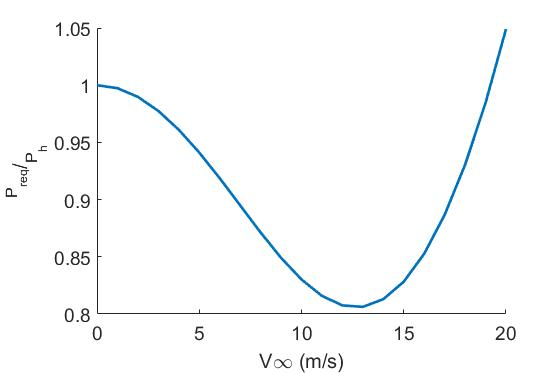
\includegraphics[width=8cm]{constant-config-ratio.jpg}
% 	\caption{The ratio of power required in forward, level flight at a given velocity to power required at hover. Maximum endurance is achieved at the minimum of this curve. For the given configuration we see that flying at $V_{me}$ reduces the power required by 19 percent.}
% \end{figure}

\begin{figure}
    \centering
    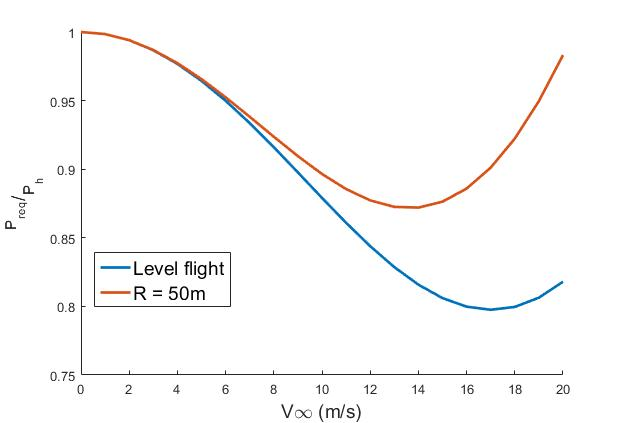
\includegraphics[width=8cm]{images/m100-turn-vs-level.jpg}
    \caption{We compare the theoretical power ratio for our vehicle configuration using momentum theory analysis. If our vehicle was flown straight and level at 17m/s we could expect to fly approximately 21\% longer. Even with losses associated with overcoming centripetal acceleration we can expect to fly 13\% longer by flying at 13m/s while turning with a radius of 50m.}
    \label{m100levelturn}
\end{figure}

\section{Optimal Control Problem}
\label{formulation}
% !TeX root = ../main.tex
 

\section{Results and Discussion}
\label{results}
% !TeX root = ../main.tex

To determine the effectiveness of a trajectory, $\mathscr{T}_c$ we empirically compare the time it takes to deplete 450 mAh of charge while flying $\mathscr{T}_c$ versus the time it takes to deplete the same charge at hover. The experiment consists of two main phases: hover flights and trajectory flights where these two phases are flown by the same quadrotor in controlled conditions. The parameters defining $\mathscr{T}_c$ (i.e. $v_Q$, $R_t$, type of yaw tracking) vary between iterations while hover parameters remain unchanged. Each iteration begins by replacing the used battery with a fully charged one, determining if local wind speeds are below moderate which we define below, and ensuring the ambient air temperature is within our bounds. The experiments were designed this way to control for two primary factors, wind and battery variations.

\subsection{Controlling for wind variations}
From equations [eqno?] and decades of aerodynamic research we know that aircraft performance is susceptible to wind disturbances. Extensive work has been done in flight control to reduce wind induced error in the absence of a human pilot. \cite{escareno2013trajectory} and \cite{waslander2009wind} focus on the quadrotor platform while \cite{mcgee2006path} looks at the more traditional fixed-wing aircraft.
In \cite{escareno2013trajectory} and \cite{mcgee2006path} wind disturbance is categorized by 
\begin{equation}
    W = \frac{\lvert V_w \rvert}{\lvert V_Q \rvert}*100\%
\end{equation}
As stated in section \ref{derivations}, in this paper we are not concerned with controlling against moderate or severe wind disturbance. Therefore, before each flight test we measure the local wind speed to ensure $W<20\%$ or below moderate conditions.

\subsection{Mitigating battery issues}


\subsection{Quadrotor platform}
For this experiment we flew the DJI Matrice 100 with an Intel NUC7i7DNHE serving as an onboard high level controller. The NUC7i7DNHE interfaces directly with the DJI ROS SDK to manage flight plans and log data. Our ROS package for interfacing with the SDK can be found at https://github.com/alex-faustino/dji-GNC-ROS.

\subsection{Measuring consumption}
The DJI SDK reports the battery's state of charge (SoC) at 10Hz. This was a major reason for selecting this platform as there is no need for additional boards or modules to measure battery consumption.

\begin{figure}[ht]
	\centering
	
\includegraphics[width=8cm]{placeholder-image.jpg}
	\caption{Graphic detailing setup.}
\end{figure}


\section{Conclusions and Future Work}
\label{conclusion}
% !TeX root = ../main.tex

INSERT CONCLUSIONS HERE.

%%%%%%%%%%%%%%%%%%%%%%%%%%%%%%%%%%%%%%%%%%%%%%%%%%%%%%%%%%%%%%%%%%%%%%%%%%%%%%%%

%\addtolength{\textheight}{-12cm}   % needs to be before last page to work

%%%%%%%%%%%%%%%%%%%%%%%%%%%%%%%%%%%%%%%%%%%%%%%%%%%%%%%%%%%%%%%%%%%%%%%%%%%%%%%%
\section*{APPENDIX}

Appendixes should appear before the acknowledgment.

\section*{ACKNOWLEDGMENT}

Enter shout outs here.

\bibliographystyle{IEEEtran}
\bibliography{sections/references}

\end{document}
